\documentclass[aspectratio=169]{beamer}

% Theme and basics
\usetheme{Madrid}
\usecolortheme{default}
\usefonttheme{professionalfonts}
\setbeamertemplate{navigation symbols}{}

% Custom footline: short author and short title on all non-title slides
\setbeamertemplate{footline}{%
  \leavevmode
  \hbox{%
    \begin{beamercolorbox}[wd=\paperwidth,ht=2.5ex,dp=1ex,center]{author in head/foot}
      \usebeamerfont{author in head/foot}\insertshortauthor\,\textemdash\,\insertshorttitle
    \end{beamercolorbox}%
  }%
}

% Math and utilities
\usepackage{amsmath,amssymb,amsfonts}
\usepackage{bm}
\usepackage{graphicx}
\usepackage{subcaption}
\usepackage{booktabs}
\usepackage{tabularx}
\usepackage{arydshln}
\usepackage{array}
\usepackage{mathtools}
\usepackage{hyperref}
\usepackage{cleveref}
\usepackage{fontawesome5} % for question mark
%\usepackage[authoryear]{natbib}

\usepackage{environ}
\newcounter{aequation}
\NewEnviron{aequation}{\refstepcounter{aequation}$$\BODY\eqno{\text{(A\theaequation)}}$$}
\crefname{aequation}{assumption}{assumptions}
\creflabelformat{aequation}{(#2A#1#3)}


% Citations use the standard natbib formatting (as in the article)
\usepackage[style=authoryear, maxcitenames=1, maxbibnames=3, terseinits=true, uniquelist=false, natbib=true,]{biblatex}
\addbibresource{../conf_article/icomp2024_conference.bib}
% Reuse article macros
%%%%% NEW MATH DEFINITIONS %%%%%

\usepackage{amsmath,amsfonts,bm}

% Mark sections of captions for referring to divisions of figures
\newcommand{\figleft}{{\em (Left)}}
\newcommand{\figcenter}{{\em (Center)}}
\newcommand{\figright}{{\em (Right)}}
\newcommand{\figtop}{{\em (Top)}}
\newcommand{\figbottom}{{\em (Bottom)}}
\newcommand{\captiona}{{\em (a)}}
\newcommand{\captionb}{{\em (b)}}
\newcommand{\captionc}{{\em (c)}}
\newcommand{\captiond}{{\em (d)}}

% Highlight a newly defined term
\newcommand{\newterm}[1]{{\bf #1}}


% Figure reference, lower-case.
\def\figref#1{figure~\ref{#1}}
% Figure reference, capital. For start of sentence
\def\Figref#1{Figure~\ref{#1}}
\def\twofigref#1#2{figures \ref{#1} and \ref{#2}}
\def\quadfigref#1#2#3#4{figures \ref{#1}, \ref{#2}, \ref{#3} and \ref{#4}}
% Section reference, lower-case.
\def\secref#1{section~\ref{#1}}
% Section reference, capital.
\def\Secref#1{Section~\ref{#1}}
% Reference to two sections.
\def\twosecrefs#1#2{sections \ref{#1} and \ref{#2}}
% Reference to three sections.
\def\secrefs#1#2#3{sections \ref{#1}, \ref{#2} and \ref{#3}}
% Reference to an equation, lower-case.
\def\eqref#1{equation~\ref{#1}}
% Reference to an equation, upper case
\def\Eqref#1{Equation~\ref{#1}}
% A raw reference to an equation---avoid using if possible
\def\plaineqref#1{\ref{#1}}
% Reference to a chapter, lower-case.
\def\chapref#1{chapter~\ref{#1}}
% Reference to an equation, upper case.
\def\Chapref#1{Chapter~\ref{#1}}
% Reference to a range of chapters
\def\rangechapref#1#2{chapters\ref{#1}--\ref{#2}}
% Reference to an algorithm, lower-case.
\def\algref#1{algorithm~\ref{#1}}
% Reference to an algorithm, upper case.
\def\Algref#1{Algorithm~\ref{#1}}
\def\twoalgref#1#2{algorithms \ref{#1} and \ref{#2}}
\def\Twoalgref#1#2{Algorithms \ref{#1} and \ref{#2}}
% Reference to a part, lower case
\def\partref#1{part~\ref{#1}}
% Reference to a part, upper case
\def\Partref#1{Part~\ref{#1}}
\def\twopartref#1#2{parts \ref{#1} and \ref{#2}}

\def\ceil#1{\lceil #1 \rceil}
\def\floor#1{\lfloor #1 \rfloor}
\def\1{\bm{1}}
\newcommand{\train}{\mathcal{D}}
\newcommand{\valid}{\mathcal{D_{\mathrm{valid}}}}
\newcommand{\test}{\mathcal{D_{\mathrm{test}}}}

\def\eps{{\epsilon}}


% Random variables
\def\reta{{\textnormal{$\eta$}}}
\def\ra{{\textnormal{a}}}
\def\rb{{\textnormal{b}}}
\def\rc{{\textnormal{c}}}
\def\rd{{\textnormal{d}}}
\def\re{{\textnormal{e}}}
\def\rf{{\textnormal{f}}}
\def\rg{{\textnormal{g}}}
\def\rh{{\textnormal{h}}}
\def\ri{{\textnormal{i}}}
\def\rj{{\textnormal{j}}}
\def\rk{{\textnormal{k}}}
\def\rl{{\textnormal{l}}}
% rm is already a command, just don't name any random variables m
\def\rn{{\textnormal{n}}}
\def\ro{{\textnormal{o}}}
\def\rp{{\textnormal{p}}}
\def\rq{{\textnormal{q}}}
\def\rr{{\textnormal{r}}}
\def\rs{{\textnormal{s}}}
\def\rt{{\textnormal{t}}}
\def\ru{{\textnormal{u}}}
\def\rv{{\textnormal{v}}}
\def\rw{{\textnormal{w}}}
\def\rx{{\textnormal{x}}}
\def\ry{{\textnormal{y}}}
\def\rz{{\textnormal{z}}}

% Random vectors
\def\rvepsilon{{\mathbf{\epsilon}}}
\def\rvtheta{{\mathbf{\theta}}}
\def\rva{{\mathbf{a}}}
\def\rvb{{\mathbf{b}}}
\def\rvc{{\mathbf{c}}}
\def\rvd{{\mathbf{d}}}
\def\rve{{\mathbf{e}}}
\def\rvf{{\mathbf{f}}}
\def\rvg{{\mathbf{g}}}
\def\rvh{{\mathbf{h}}}
\def\rvu{{\mathbf{i}}}
\def\rvj{{\mathbf{j}}}
\def\rvk{{\mathbf{k}}}
\def\rvl{{\mathbf{l}}}
\def\rvm{{\mathbf{m}}}
\def\rvn{{\mathbf{n}}}
\def\rvo{{\mathbf{o}}}
\def\rvp{{\mathbf{p}}}
\def\rvq{{\mathbf{q}}}
\def\rvr{{\mathbf{r}}}
\def\rvs{{\mathbf{s}}}
\def\rvt{{\mathbf{t}}}
\def\rvu{{\mathbf{u}}}
\def\rvv{{\mathbf{v}}}
\def\rvw{{\mathbf{w}}}
\def\rvx{{\mathbf{x}}}
\def\rvy{{\mathbf{y}}}
\def\rvz{{\mathbf{z}}}

% Elements of random vectors
\def\erva{{\textnormal{a}}}
\def\ervb{{\textnormal{b}}}
\def\ervc{{\textnormal{c}}}
\def\ervd{{\textnormal{d}}}
\def\erve{{\textnormal{e}}}
\def\ervf{{\textnormal{f}}}
\def\ervg{{\textnormal{g}}}
\def\ervh{{\textnormal{h}}}
\def\ervi{{\textnormal{i}}}
\def\ervj{{\textnormal{j}}}
\def\ervk{{\textnormal{k}}}
\def\ervl{{\textnormal{l}}}
\def\ervm{{\textnormal{m}}}
\def\ervn{{\textnormal{n}}}
\def\ervo{{\textnormal{o}}}
\def\ervp{{\textnormal{p}}}
\def\ervq{{\textnormal{q}}}
\def\ervr{{\textnormal{r}}}
\def\ervs{{\textnormal{s}}}
\def\ervt{{\textnormal{t}}}
\def\ervu{{\textnormal{u}}}
\def\ervv{{\textnormal{v}}}
\def\ervw{{\textnormal{w}}}
\def\ervx{{\textnormal{x}}}
\def\ervy{{\textnormal{y}}}
\def\ervz{{\textnormal{z}}}

% Random matrices
\def\rmA{{\mathbf{A}}}
\def\rmB{{\mathbf{B}}}
\def\rmC{{\mathbf{C}}}
\def\rmD{{\mathbf{D}}}
\def\rmE{{\mathbf{E}}}
\def\rmF{{\mathbf{F}}}
\def\rmG{{\mathbf{G}}}
\def\rmH{{\mathbf{H}}}
\def\rmI{{\mathbf{I}}}
\def\rmJ{{\mathbf{J}}}
\def\rmK{{\mathbf{K}}}
\def\rmL{{\mathbf{L}}}
\def\rmM{{\mathbf{M}}}
\def\rmN{{\mathbf{N}}}
\def\rmO{{\mathbf{O}}}
\def\rmP{{\mathbf{P}}}
\def\rmQ{{\mathbf{Q}}}
\def\rmR{{\mathbf{R}}}
\def\rmS{{\mathbf{S}}}
\def\rmT{{\mathbf{T}}}
\def\rmU{{\mathbf{U}}}
\def\rmV{{\mathbf{V}}}
\def\rmW{{\mathbf{W}}}
\def\rmX{{\mathbf{X}}}
\def\rmY{{\mathbf{Y}}}
\def\rmZ{{\mathbf{Z}}}

% Elements of random matrices
\def\ermA{{\textnormal{A}}}
\def\ermB{{\textnormal{B}}}
\def\ermC{{\textnormal{C}}}
\def\ermD{{\textnormal{D}}}
\def\ermE{{\textnormal{E}}}
\def\ermF{{\textnormal{F}}}
\def\ermG{{\textnormal{G}}}
\def\ermH{{\textnormal{H}}}
\def\ermI{{\textnormal{I}}}
\def\ermJ{{\textnormal{J}}}
\def\ermK{{\textnormal{K}}}
\def\ermL{{\textnormal{L}}}
\def\ermM{{\textnormal{M}}}
\def\ermN{{\textnormal{N}}}
\def\ermO{{\textnormal{O}}}
\def\ermP{{\textnormal{P}}}
\def\ermQ{{\textnormal{Q}}}
\def\ermR{{\textnormal{R}}}
\def\ermS{{\textnormal{S}}}
\def\ermT{{\textnormal{T}}}
\def\ermU{{\textnormal{U}}}
\def\ermV{{\textnormal{V}}}
\def\ermW{{\textnormal{W}}}
\def\ermX{{\textnormal{X}}}
\def\ermY{{\textnormal{Y}}}
\def\ermZ{{\textnormal{Z}}}

% Vectors
\def\vzero{{\bm{0}}}
\def\vone{{\bm{1}}}
\def\vmu{{\bm{\mu}}}
\def\vtheta{{\bm{\theta}}}
\def\va{{\bm{a}}}
\def\vb{{\bm{b}}}
\def\vc{{\bm{c}}}
\def\vd{{\bm{d}}}
\def\ve{{\bm{e}}}
\def\vf{{\bm{f}}}
\def\vg{{\bm{g}}}
\def\vh{{\bm{h}}}
\def\vi{{\bm{i}}}
\def\vj{{\bm{j}}}
\def\vk{{\bm{k}}}
\def\vl{{\bm{l}}}
\def\vm{{\bm{m}}}
\def\vn{{\bm{n}}}
\def\vo{{\bm{o}}}
\def\vp{{\bm{p}}}
\def\vq{{\bm{q}}}
\def\vr{{\bm{r}}}
\def\vs{{\bm{s}}}
\def\vt{{\bm{t}}}
\def\vu{{\bm{u}}}
\def\vv{{\bm{v}}}
\def\vw{{\bm{w}}}
\def\vx{{\bm{x}}}
\def\vy{{\bm{y}}}
\def\vz{{\bm{z}}}

% Elements of vectors
\def\evalpha{{\alpha}}
\def\evbeta{{\beta}}
\def\evepsilon{{\epsilon}}
\def\evlambda{{\lambda}}
\def\evomega{{\omega}}
\def\evmu{{\mu}}
\def\evpsi{{\psi}}
\def\evsigma{{\sigma}}
\def\evtheta{{\theta}}
\def\eva{{a}}
\def\evb{{b}}
\def\evc{{c}}
\def\evd{{d}}
\def\eve{{e}}
\def\evf{{f}}
\def\evg{{g}}
\def\evh{{h}}
\def\evi{{i}}
\def\evj{{j}}
\def\evk{{k}}
\def\evl{{l}}
\def\evm{{m}}
\def\evn{{n}}
\def\evo{{o}}
\def\evp{{p}}
\def\evq{{q}}
\def\evr{{r}}
\def\evs{{s}}
\def\evt{{t}}
\def\evu{{u}}
\def\evv{{v}}
\def\evw{{w}}
\def\evx{{x}}
\def\evy{{y}}
\def\evz{{z}}

% Matrix
\def\mA{{\bm{A}}}
\def\mB{{\bm{B}}}
\def\mC{{\bm{C}}}
\def\mD{{\bm{D}}}
\def\mE{{\bm{E}}}
\def\mF{{\bm{F}}}
\def\mG{{\bm{G}}}
\def\mH{{\bm{H}}}
\def\mI{{\bm{I}}}
\def\mJ{{\bm{J}}}
\def\mK{{\bm{K}}}
\def\mL{{\bm{L}}}
\def\mM{{\bm{M}}}
\def\mN{{\bm{N}}}
\def\mO{{\bm{O}}}
\def\mP{{\bm{P}}}
\def\mQ{{\bm{Q}}}
\def\mR{{\bm{R}}}
\def\mS{{\bm{S}}}
\def\mT{{\bm{T}}}
\def\mU{{\bm{U}}}
\def\mV{{\bm{V}}}
\def\mW{{\bm{W}}}
\def\mX{{\bm{X}}}
\def\mY{{\bm{Y}}}
\def\mZ{{\bm{Z}}}
\def\mBeta{{\bm{\beta}}}
\def\mPhi{{\bm{\Phi}}}
\def\mLambda{{\bm{\Lambda}}}
\def\mSigma{{\bm{\Sigma}}}

% Tensor
\DeclareMathAlphabet{\mathsfit}{\encodingdefault}{\sfdefault}{m}{sl}
\SetMathAlphabet{\mathsfit}{bold}{\encodingdefault}{\sfdefault}{bx}{n}
\newcommand{\tens}[1]{\bm{\mathsfit{#1}}}
\def\tA{{\tens{A}}}
\def\tB{{\tens{B}}}
\def\tC{{\tens{C}}}
\def\tD{{\tens{D}}}
\def\tE{{\tens{E}}}
\def\tF{{\tens{F}}}
\def\tG{{\tens{G}}}
\def\tH{{\tens{H}}}
\def\tI{{\tens{I}}}
\def\tJ{{\tens{J}}}
\def\tK{{\tens{K}}}
\def\tL{{\tens{L}}}
\def\tM{{\tens{M}}}
\def\tN{{\tens{N}}}
\def\tO{{\tens{O}}}
\def\tP{{\tens{P}}}
\def\tQ{{\tens{Q}}}
\def\tR{{\tens{R}}}
\def\tS{{\tens{S}}}
\def\tT{{\tens{T}}}
\def\tU{{\tens{U}}}
\def\tV{{\tens{V}}}
\def\tW{{\tens{W}}}
\def\tX{{\tens{X}}}
\def\tY{{\tens{Y}}}
\def\tZ{{\tens{Z}}}


% Graph
\def\gA{{\mathcal{A}}}
\def\gB{{\mathcal{B}}}
\def\gC{{\mathcal{C}}}
\def\gD{{\mathcal{D}}}
\def\gE{{\mathcal{E}}}
\def\gF{{\mathcal{F}}}
\def\gG{{\mathcal{G}}}
\def\gH{{\mathcal{H}}}
\def\gI{{\mathcal{I}}}
\def\gJ{{\mathcal{J}}}
\def\gK{{\mathcal{K}}}
\def\gL{{\mathcal{L}}}
\def\gM{{\mathcal{M}}}
\def\gN{{\mathcal{N}}}
\def\gO{{\mathcal{O}}}
\def\gP{{\mathcal{P}}}
\def\gQ{{\mathcal{Q}}}
\def\gR{{\mathcal{R}}}
\def\gS{{\mathcal{S}}}
\def\gT{{\mathcal{T}}}
\def\gU{{\mathcal{U}}}
\def\gV{{\mathcal{V}}}
\def\gW{{\mathcal{W}}}
\def\gX{{\mathcal{X}}}
\def\gY{{\mathcal{Y}}}
\def\gZ{{\mathcal{Z}}}

% Sets
\def\sA{{\mathbb{A}}}
\def\sB{{\mathbb{B}}}
\def\sC{{\mathbb{C}}}
\def\sD{{\mathbb{D}}}
% Don't use a set called E, because this would be the same as our symbol
% for expectation.
\def\sF{{\mathbb{F}}}
\def\sG{{\mathbb{G}}}
\def\sH{{\mathbb{H}}}
\def\sI{{\mathbb{I}}}
\def\sJ{{\mathbb{J}}}
\def\sK{{\mathbb{K}}}
\def\sL{{\mathbb{L}}}
\def\sM{{\mathbb{M}}}
\def\sN{{\mathbb{N}}}
\def\sO{{\mathbb{O}}}
\def\sP{{\mathbb{P}}}
\def\sQ{{\mathbb{Q}}}
\def\sR{{\mathbb{R}}}
\def\sS{{\mathbb{S}}}
\def\sT{{\mathbb{T}}}
\def\sU{{\mathbb{U}}}
\def\sV{{\mathbb{V}}}
\def\sW{{\mathbb{W}}}
\def\sX{{\mathbb{X}}}
\def\sY{{\mathbb{Y}}}
\def\sZ{{\mathbb{Z}}}

% Entries of a matrix
\def\emLambda{{\Lambda}}
\def\emA{{A}}
\def\emB{{B}}
\def\emC{{C}}
\def\emD{{D}}
\def\emE{{E}}
\def\emF{{F}}
\def\emG{{G}}
\def\emH{{H}}
\def\emI{{I}}
\def\emJ{{J}}
\def\emK{{K}}
\def\emL{{L}}
\def\emM{{M}}
\def\emN{{N}}
\def\emO{{O}}
\def\emP{{P}}
\def\emQ{{Q}}
\def\emR{{R}}
\def\emS{{S}}
\def\emT{{T}}
\def\emU{{U}}
\def\emV{{V}}
\def\emW{{W}}
\def\emX{{X}}
\def\emY{{Y}}
\def\emZ{{Z}}
\def\emSigma{{\Sigma}}

% entries of a tensor
% Same font as tensor, without \bm wrapper
\newcommand{\etens}[1]{\mathsfit{#1}}
\def\etLambda{{\etens{\Lambda}}}
\def\etA{{\etens{A}}}
\def\etB{{\etens{B}}}
\def\etC{{\etens{C}}}
\def\etD{{\etens{D}}}
\def\etE{{\etens{E}}}
\def\etF{{\etens{F}}}
\def\etG{{\etens{G}}}
\def\etH{{\etens{H}}}
\def\etI{{\etens{I}}}
\def\etJ{{\etens{J}}}
\def\etK{{\etens{K}}}
\def\etL{{\etens{L}}}
\def\etM{{\etens{M}}}
\def\etN{{\etens{N}}}
\def\etO{{\etens{O}}}
\def\etP{{\etens{P}}}
\def\etQ{{\etens{Q}}}
\def\etR{{\etens{R}}}
\def\etS{{\etens{S}}}
\def\etT{{\etens{T}}}
\def\etU{{\etens{U}}}
\def\etV{{\etens{V}}}
\def\etW{{\etens{W}}}
\def\etX{{\etens{X}}}
\def\etY{{\etens{Y}}}
\def\etZ{{\etens{Z}}}

% The true underlying data generating distribution
\newcommand{\pdata}{p_{\rm{data}}}
% The empirical distribution defined by the training set
\newcommand{\ptrain}{\hat{p}_{\rm{data}}}
\newcommand{\Ptrain}{\hat{P}_{\rm{data}}}
% The model distribution
\newcommand{\pmodel}{p_{\rm{model}}}
\newcommand{\Pmodel}{P_{\rm{model}}}
\newcommand{\ptildemodel}{\tilde{p}_{\rm{model}}}
% Stochastic autoencoder distributions
\newcommand{\pencode}{p_{\rm{encoder}}}
\newcommand{\pdecode}{p_{\rm{decoder}}}
\newcommand{\precons}{p_{\rm{reconstruct}}}

\newcommand{\laplace}{\mathrm{Laplace}} % Laplace distribution

\newcommand{\E}{\mathbb{E}}
\newcommand{\Ls}{\mathcal{L}}
\newcommand{\R}{\mathbb{R}}
\newcommand{\emp}{\tilde{p}}
\newcommand{\lr}{\alpha}
\newcommand{\reg}{\lambda}
\newcommand{\rect}{\mathrm{rectifier}}
\newcommand{\softmax}{\mathrm{softmax}}
\newcommand{\sigmoid}{\sigma}
\newcommand{\softplus}{\zeta}
\newcommand{\KL}{D_{\mathrm{KL}}}
\newcommand{\Var}{\mathrm{Var}}
\newcommand{\standarderror}{\mathrm{SE}}
\newcommand{\Cov}{\mathrm{Cov}}
% Wolfram Mathworld says $L^2$ is for function spaces and $\ell^2$ is for vectors
% But then they seem to use $L^2$ for vectors throughout the site, and so does
% wikipedia.
\newcommand{\normlzero}{L^0}
\newcommand{\normlone}{L^1}
\newcommand{\normltwo}{L^2}
\newcommand{\normlp}{L^p}
\newcommand{\normmax}{L^\infty}

\newcommand{\parents}{Pa} % See usage in notation.tex. Chosen to match Daphne's book.

\DeclareMathOperator*{\argmax}{arg\,max}
\DeclareMathOperator*{\argmin}{arg\,min}

\DeclareMathOperator{\sign}{sign}
\DeclareMathOperator{\Tr}{Tr}
\let\ab\allowbreak


\newcommand{\norm}[1]{\lVert #1\rVert}
\newcommand{\abs}[1]{\lvert #1 \rvert}

% \epsilon is predefined; override to use \varepsilon
\renewcommand{\epsilon}{\varepsilon}
\newcommand{\Rmn}{\R^{m\times n}}
\newcommand{\cB}{\mathcal{B}}
\newcommand{\cD}{\mathcal{D}}
\newcommand{\cN}{\mathcal{N}}
\newcommand{\cO}{\mathcal{O}}
\newcommand{\cS}{\mathcal{S}}
\newcommand{\Ed}[2]{\mathbb{E}_{#1}\left[#2\right]}
\usepackage{mathtools}
\DeclarePairedDelimiter{\sqne}{\|}{\|_2^2}
%\DeclarePairedDelimiter{\norme}{\|}{\|_2}
\DeclarePairedDelimiter{\normf}{\|}{\|_\mathrm{F}}
\DeclarePairedDelimiter{\normkfk}{\|}{\|_\mathrm{KF-k}}
\DeclarePairedDelimiter{\normfstar}{\|}{\|_\mathrm{F*}}
\DeclarePairedDelimiter{\normftwo}{\|}{\|_\mathrm{F2}}
\DeclarePairedDelimiter{\sqns}{\|}{\|_{\mathrm{op}}^2}
\DeclarePairedDelimiter{\norms}{\|}{\|_{\mathrm{op}}}
\DeclarePairedDelimiter{\sqnn}{\|}{\|_{\mathrm{nuc}}^2}
\DeclarePairedDelimiter{\sqnf}{\|}{\|_{\mathrm{F}}^2}
\DeclarePairedDelimiter{\normn}{\|}{\|_{\mathrm{nuc}}}
\DeclarePairedDelimiter{\normfkfk}{\|}{\|_{\mathrm{F-KF-k}}}
\def\<#1,#2>{\langle #1,#2\rangle}
\DeclarePairedDelimiter{\dotprod}{\langle}{\rangle}

\DeclareMathOperator{\tr}{tr}
\DeclareMathOperator{\diag}{diag}

% Graphics from the article repo
\graphicspath{{../conf_article/figs/}{../figures/13may_muon_neon/}}

% Title
\title[The Ky Fan Norms and Beyond]{The Ky Fan Norms and Beyond: Dual Norms and Combinations for Matrix Optimization}
\author[A. Kravatskiy et al.]{%
  Alexey Kravatskiy\inst{1} \and
  Ivan Kozyrev\inst{1} \and
  Nikolai Kozlov\inst{1} \and
  Alexander Vinogradov\inst{1} \and
  Daniil Merkulov\inst{1,2,3,4} \and
  Ivan Oseledets\inst{5,2}\\[0.3em]
}
\institute[]{%
\inst{1} MIPT \hspace{1em}%
\inst{2} Skoltech \hspace{1em}%
\inst{3} HSE \hspace{1em}%
\inst{4} AI4Science \hspace{1em}%
\inst{5} AIRI
}
\date{\today}

\begin{document}

%-------------------------------------------------------------------------------------
\begin{frame}[plain]
  \titlepage
\end{frame}
%-------------------------------------------------------------------------------------
\begin{frame}{Moving beyond the spectral norm and Muon}
    \begin{block}{Objective:  $\min_{\mX\in\R^{m\times n}} f(\mX)$}
    \faQuestionCircle \space What will happen if we change the spectral norm in the derivation of Muon?
    \end{block}
    \begin{block}{F-Fanions: Muon, Neon, NSGD, Dion without EF, and so much more}
        From $\norms{\cdot}$ and Muon:
        $$\mX^{t+1} = \mX^{t} - \eta U V^\top$$
        To $\normkfk{\cdot}^\dagger$ and a general F-Fanion:
        $$\mX^{t+1} = \mX^{t} - \eta \left(\alpha \sum_{i=1}^k{u_i v_i^\top} + (1-\alpha)\frac{\mM^t}{\normf{\mM^t}}\right), \alpha \in [0,1]$$
    \end{block}
      
\end{frame}
%-------------------------------------------------------------------------------------
\begin{frame}{Linear Minimization Oracle (LMO) and Trust Region}
% after omitting gamma_k, we obtain:
Let us equip $\Rmn$ with a norm $\norm{\cdot}$. Its dual is $\norm{\mX}^\dagger = \sup_{\norm{\mX'}\leq 1} \<\mX,\mX'>$. $\<\cdot, \cdot>$ is a Frobenius product.
\vspace{0.4em}

Both LMO and Trust Region lead to the update
$$\mX^{t+1} = \mX^{t} - \eta \arg\max_{\mX \in \cB_1} \<\mM^t, \mX> = \mX^{t} - \eta \{\Delta \in \cB_1 \mid \<\mM^t, \Delta> = \norm{\mM^t}^\dagger\}$$

\vspace{0.4em}

\textbf{Recipe}: It means we seek $\Delta$ from the 1-norm ball that delivers $\<\mM^t, \Delta> = \norm{\mM^t}^\dagger$. We will often return to the SVD $\mM^t = \mU \Sigma \mV^\top$.
\end{frame}
%-------------------------------------------------------------------------------------
\begin{frame}{Frobenius $\normf{\mM^{k}}$ and Normalized SGD}

\begin{block}{Deriving NSGD by Recipe} $\normf{\mM^t}^\dagger = \normf{\mM^t}$, and $\Delta = \frac{\mM^t}{\normf{\mM^t}}$ with $\normf{\Delta} = 1$ delivers it. Hence,
$$\mX^{t+1} = \mX^{t} - \eta \frac{\mM^t}{\normf{\mM^t}}$$
\end{block}
\end{frame}
%-------------------------------------------------------------------------------------
\begin{frame}{Spectral $\norms{\mM^{k}}$ and Muon. Nuclear $\normn{\mM^k}$ and Neon.}
\begin{block}{Deriving Muon by Recipe} $\norms{\mM^t}^\dagger = \normn{\mM^t}$, and $\Delta = \mU\mV^\top$ delivers it: $\norms{\Delta}$ = 1 and

$$\<\mU\Sigma\mV^\top, \mU\mV^\top> = \tr(\mV \Sigma \mU^\top \mU \mV^\top) = \tr\Sigma = \normn{\mM^t}$$

Hence,
$$\mX^{t+1} = \mX^{t} - \eta \mU \mV^\top$$

\end{block}

\begin{block}{Deriving Neon by Recipe} $\normn{\mM^t}^\dagger = \norms{\mM^t}$, and $\Delta = u_1 v_1^\top$ delivers it: $\normn{\Delta}$ = 1 and

$$\<\mU\Sigma\mV^\top, u_1 v_1^\top> = \tr(\mV \Sigma \mU^\top u_1 v_1^\top) = \tr\diag({\sigma_1, 0, \dots, 0}) = \sigma_1 = \norms{\mM^t}$$

Hence,
$$\mX^{t+1} = \mX^{t} - \eta u_1 v_1^\top$$
\end{block}
\end{frame}

%-------------------------------------------------------------------------------------
\begin{frame}{Of Matrix and Vector Algorithms}
    %\centering
    %\def\arraystretch{1.1}
    \footnotesize
    \begin{table}
    \caption{lmo optimizers in Schatten $S_p$ norms and in $l_p$ norms.}
    \label{tbl:mat_vs_vec_lmo}
    \begin{tabularx}{\linewidth}{|>{\raggedright\arraybackslash}X|c|c|c|}
    \hline
    Method & lmo constraint set $\mathcal D$ & lmo & Reference \\
    \hline\hline
    Normalized SGD & $l_2$-ball, $S_2$-ball & $-\eta \tfrac{g}{\norm{g}_2} = -\eta \tfrac{g}{\norm{g}_F}$ & \citep{hazan2015beyond} \\
    Momentum Normalized SGD & Ball in $l_2$, or Ball in $S_2$ & $-\eta \tfrac{g}{\norm{g}_2} = -\eta\tfrac{g}{\norm{g}_F}$ & \citep{cutkosky2020momentum}\\
    \hline
    SignSGD & Ball in Max-norm $l_\infty$ & $-\eta \sign(g)$ & \citep[Thm. 1]{bernstein2018signsgd} \\
    Signum  & Ball in Max-norm $l_\infty$ & $-\eta \sign(g)$ & \citep[Thm. 3]{bernstein2018signsgd} \\
    \hdashline
    Muon & Ball in Spectral $S_\infty$ & $-\eta UV^\top$ & \citep{jordan2024muon} \\
    \hline
    Gauss-Southwell Coordinate Descent & Ball in $l_1$ & $-\eta \{i: g_i \geq g_k \forall k\}$ & \citep[p.19]{shi2016primer}\\
    \hdashline 
    Neon & Ball in Nuclear $S_1$ & $-\eta u_1 v_1^\top$ & This work\\
    \hline
    \end{tabularx}
    \end{table}
\end{frame}
%------------------------------------------------------------------------------------------------------------
\begin{frame}{Understanding Dion by Thomas Pethick}
    Without momentum, Dion is simplified to
    $$
    \begin{aligned}
    \Delta &\leftarrow g + e  \\
    e &\leftarrow \Delta - \sum_{i=1}^r \sigma_i u_i v_i^\top \\
    x &\leftarrow x - \gamma \sum_{i=1}^r u_i v_i^\top
    \end{aligned}
    $$
    where $\gamma > 0$ and $\sum_{i=1}^r \sigma_i u_iv^\top_i$ is the rank-$r$ truncated SVD of $\Delta \in \Rmn$.
    \vspace{0.4em}

    \faQuestionCircle \space What will we get if we try $\normkfk{\mM}:=\sum_{i=1}^r{\sigma_i}$?
    \end{frame}
%-------------------------------------------------------------------------------------
\begin{frame}{Ky Fan $k$-rank $\normkfk{\mM^k}^\dagger$ and Fanions}

\begin{block}{Deriving Fanions by Recipe} $\normkfk{\mM^t}^{\dagger\dagger} = \normkfk{\mM^t}$, and $\Delta = \sum_{i=1}^k{u_i v_i^\top}$ with $\normkfk{\Delta}^\dagger = \max\{\frac{1}{k} \normn{\Delta}, \norms{\Delta}\} = \max\{\frac{1}{k} k, 1\} = 1$ delivers it:
    $$\<\mM^t, \Delta> =\<\mU \mSigma \mV^\top, \sum_{i=1}^{k} u_i v_i^\top> = \sum_{i,j=1}^{r, k}\<u_i \sigma_i v_i^\top, u_j v_j^\top> = \sum_{i=1}^{k}\sigma_i = \normkfk{\mM^t}$$
    
    Hence,
    $$\mX^{t+1} = \mX^{t} - \eta \sum_{i=1}^{k} u_i v_i^\top$$
    \end{block}
\end{frame}
%-----------------------------------------------------------------------------------------------------------
\begin{frame}{Computing the $k$-rank update: Lanczos method}
    \begin{center}
    \small
    \begin{tabular}{lccc}
      \toprule
      Method & rtol & $k$ & time (s) \\
      \midrule
      Power Iterations & 0.01 & 1 & 7.7 \\
      SVDS (TRLan) & 0.01 & 1 & \textbf{0.18} \\
      PCA Low Rank (RSVD) & 0.01 & 1 & 1.15 \\
      SVDS (TRLan) & 0.01 & 10 & \textbf{0.47} \\
      PCA Low Rank (RSVD) & 0.01 & 10 & 19.4 \\
      SVDS (TRLan) & 0.01 & 100 & \textbf{1.96} \\
      PCA Low Rank (RSVD) & 0.01 & 100 & 170 \\
      \bottomrule
    \end{tabular}
    \end{center}
    \vspace{0.4em}
    \centering
    \footnotesize Comparison on a \(5000\times5000\) matrix; rtol is the relative Frobenius error of $\sum_{i=1}^{k}u_i \sigma_i v_i^\top$
  \end{frame}
%--------------------------------------------------------------------------------------------------------------
\begin{frame}{Frobeniusize the norms!}
\faExclamationCircle \space $\normf{\cdot}^\dagger = \normf{\cdot}$ is not a Ky Fan norm, so NSGD is not a Fanion.
\vspace{1em}

Let us consider the convex combination of the Ky Fan rank-$k$ norm and the Frobenius norm, which we call F-KF-k-norm: $$\norm{\cdot}_{\mathrm{F-KF-k}} = \alpha \normkfk{\cdot} + (1-\alpha)\normf{\cdot}, \alpha \in [0,1]$$

\end{frame}
%--------------------------------------------------------------------------------------------------------------

\begin{frame}{Balls of Duals to Convex Combinations of Norms}
    \begin{lemma}\label{lemma:dual_to_conv_comb}
        Let $\norm{\cdot}_{(1)}$ and $\norm{\cdot}_{(2)}$ be norms on a finite-dimensional Euclidean space, and let $\alpha,\beta \geq 0$. Define 
        $$
        \norm{x} := \alpha \norm{x}_{(1)} + \beta \norm{x}_{(2)}.
        $$
        Then the dual unit ball of $\norm{\cdot}$ satisfies
        $$
        B_{\norm{\cdot}^\dagger} 
        = \alpha B_{\norm{\cdot}_{(1)}^\dagger} + \beta B_{\norm{\cdot}_{(2)}^\dagger},
        $$
        where $+$ denotes the Minkowski sum and $B_{\norm{\cdot}_{(i)}^\dagger}$ is the unit ball of the dual norm $\norm{\cdot}_{(i)}^\dagger$.
    \end{lemma}
    
\end{frame}
%-----------------------------------------------------------------------------------------------------------
\begin{frame}{$\normfkfk{\mM^k}^\dagger$ and F-Fanions}

    \begin{block}{Deriving F-Fanions by Recipe}
    $\normfkfk{\mM^t}^{\dagger\dagger} = \normfkfk{\mM^t}$, and $\Delta = \alpha\sum_{i=1}^k{u_i v_i^\top} + (1-\alpha)\frac{\mM^k}{\normf{\mM^k}}$ delivers it:
\begin{enumerate}
    \item $\normfkfk{\Delta}^\dagger \leq 1$ because $\sum_{i=1}^k{u_i v_i^\top}$ lies in $B_{\normkfk{\cdot}}$ and $\frac{\mM^k}{\normf{\mM^k}}$ lies in $B_{\normf{\cdot}}$, so $\Delta$ lies in the Minkowski sum
    \item $\<\mM^t, \Delta> =\alpha \<\mU \mSigma \mV^\top, \sum_{i=1}^{k} u_i v_i^\top> + (1-\alpha)\<\mM^t, \frac{\mM^t}{\normf{\mM^t}}> = \alpha \sum_{i=1}^{k}\sigma_i + (1-\alpha) \normf{\mM^t}= \normfkfk{\mM^t}$
\end{enumerate}
\vspace{1em}

        Hence,
        $$\mX^{t+1} = \mX^{t} - \eta \Big(\alpha\sum_{i=1}^{k} u_i v_i^\top + (1-\alpha)\frac{\mM^t}{\normf{\mM^t}}\Big)$$
        \end{block}
\end{frame}
%------------------------------------------------------------------------------------------------------------
% The next slides were generated by Cursor
\begin{frame}{F-Muon and F-Neon}
  Convex combinations with Frobenius norm:
  \[
    \|\mX\|_{F*}=\alpha\|\mX\|_*+(1-\alpha)\|\mX\|_F,\qquad
    \|\mX\|_{F2}=\alpha\|\mX\|_{op}+(1-\alpha)\|\mX\|_F.
  \]
  Dual-induced updates:
  \[
    \text{F-Muon: }\mX^{k+1}=\mX^k-\eta\Big(\alpha\,\mU\mV^\top+(1-\alpha)\tfrac{\mM^k}{\|\mM^k\|_F}\Big),
  \]
  \[
    \text{F-Neon: }\mX^{k+1}=\mX^k-\eta\Big(\alpha\,u_1 v_1^\top+(1-\alpha)\tfrac{\mM^k}{\|\mM^k\|_F}\Big).
  \]
\end{frame}
%-----------------------------------------------------------------------------------------------
\begin{frame}{Geometric intuition: Dual balls}
    \centering
    \begin{minipage}{0.48\textwidth}
        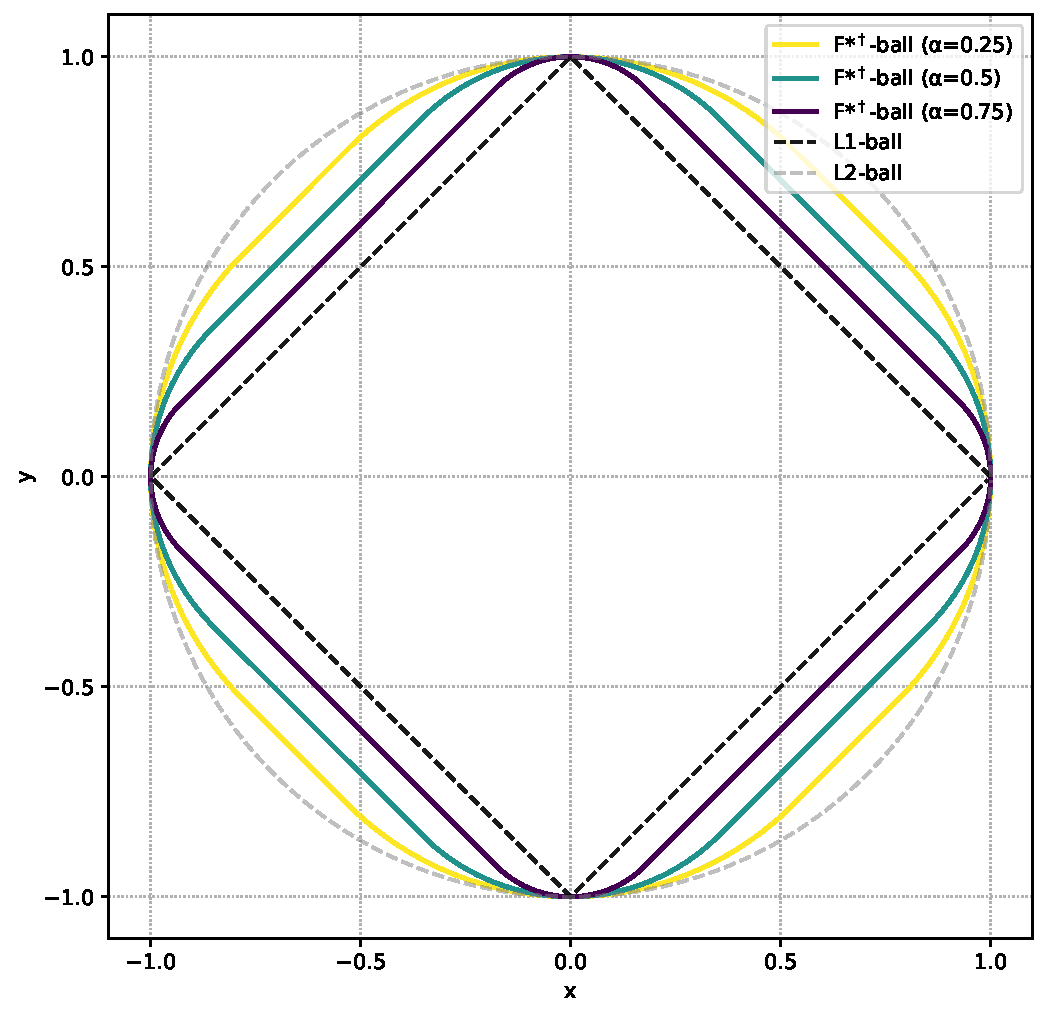
\includegraphics[height=0.75\textheight,keepaspectratio]{fstardualball.pdf}
    \end{minipage}\hfill
    \begin{minipage}{0.48\textwidth}
        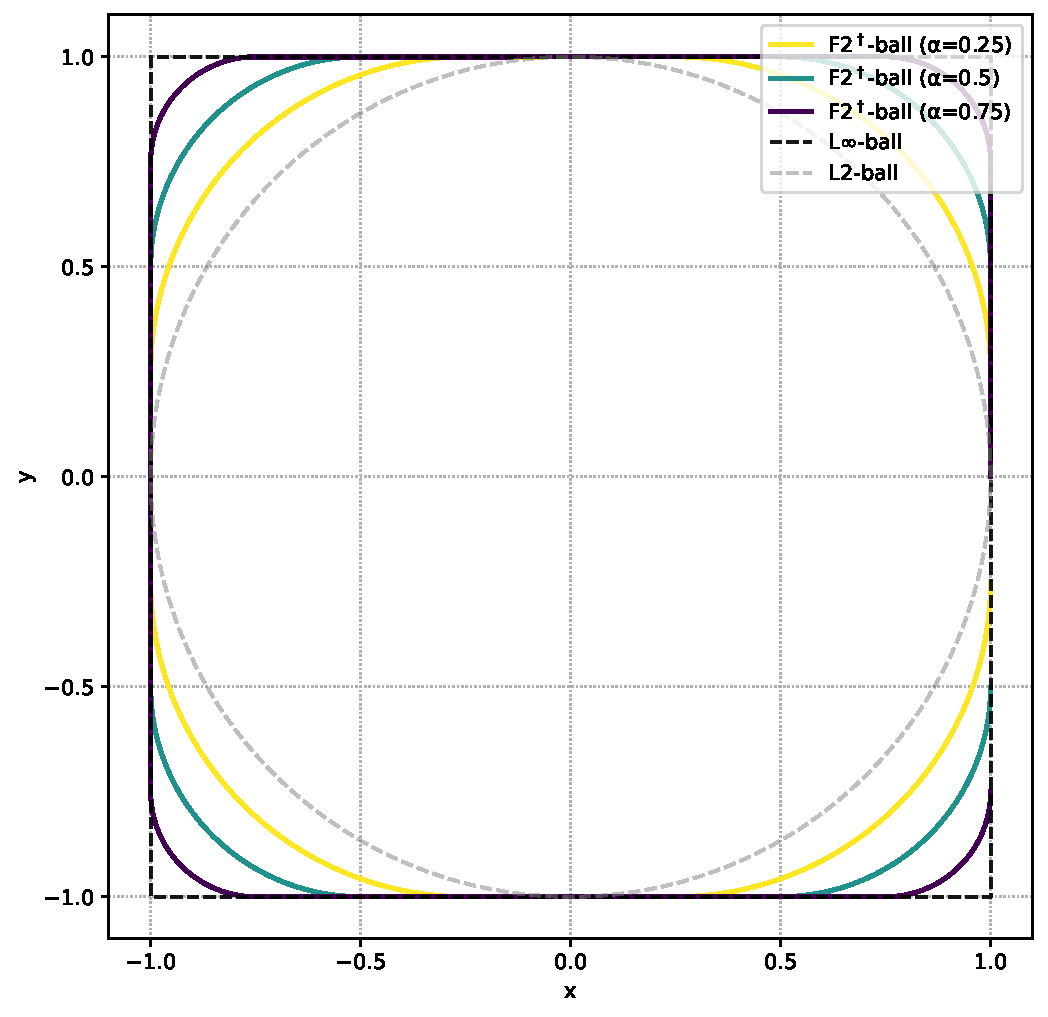
\includegraphics[height=0.75\textheight,keepaspectratio]{ftwodualball.pdf}
    \end{minipage}
    
    \vspace{0.3em}
    \footnotesize Dual balls for F-Muon and F-Neon across \(\alpha\) in a 2D singular-value space
    \end{frame}
%---------------------------------------
\begin{frame}{F-Muon on CIFAR-10 airbench}
    \begin{columns}[T,totalwidth=\textwidth]
      \begin{column}{0.48\textwidth}
        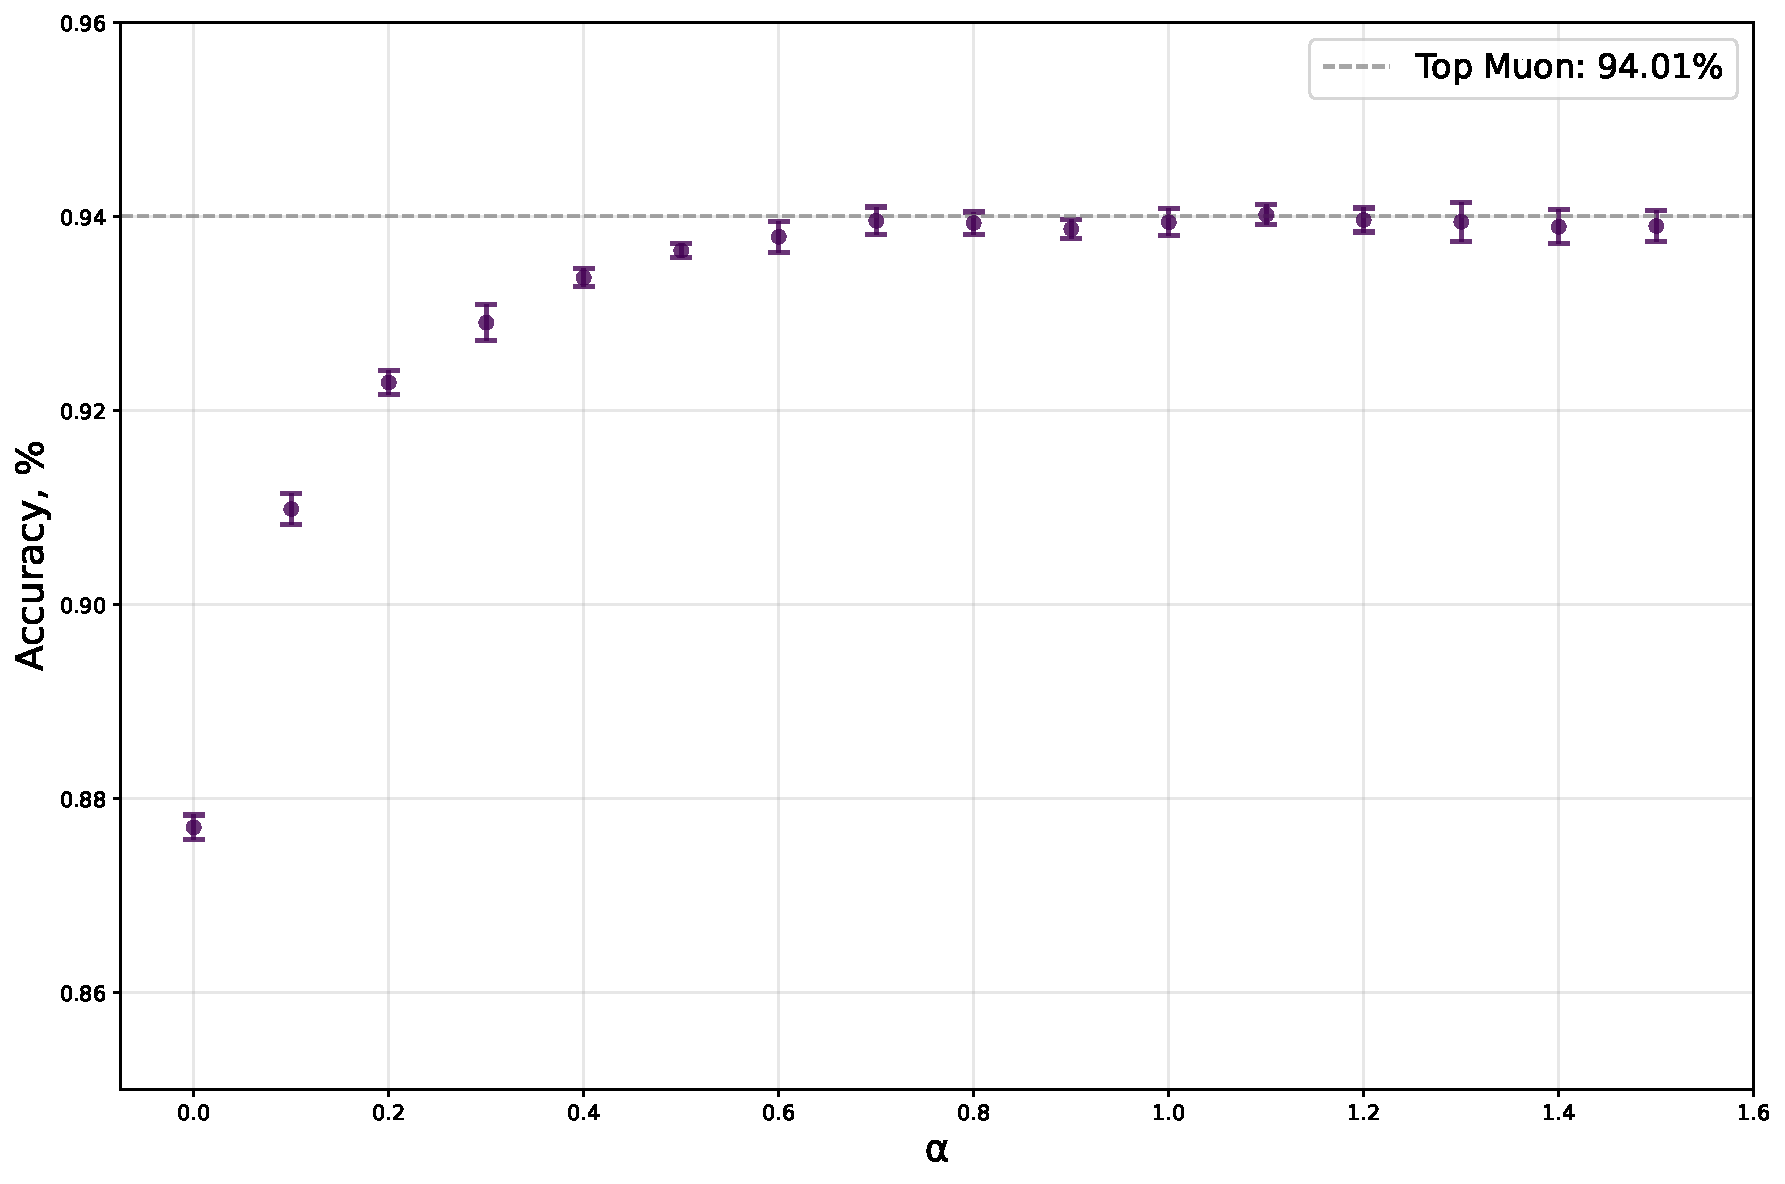
\includegraphics[width=\linewidth]{muon_tuned_diff_alpha.pdf}
        \centering
        \scriptsize With params tuned for Muon, as in \citep{cifar2023airbench}
      \end{column}
      \begin{column}{0.48\textwidth}
        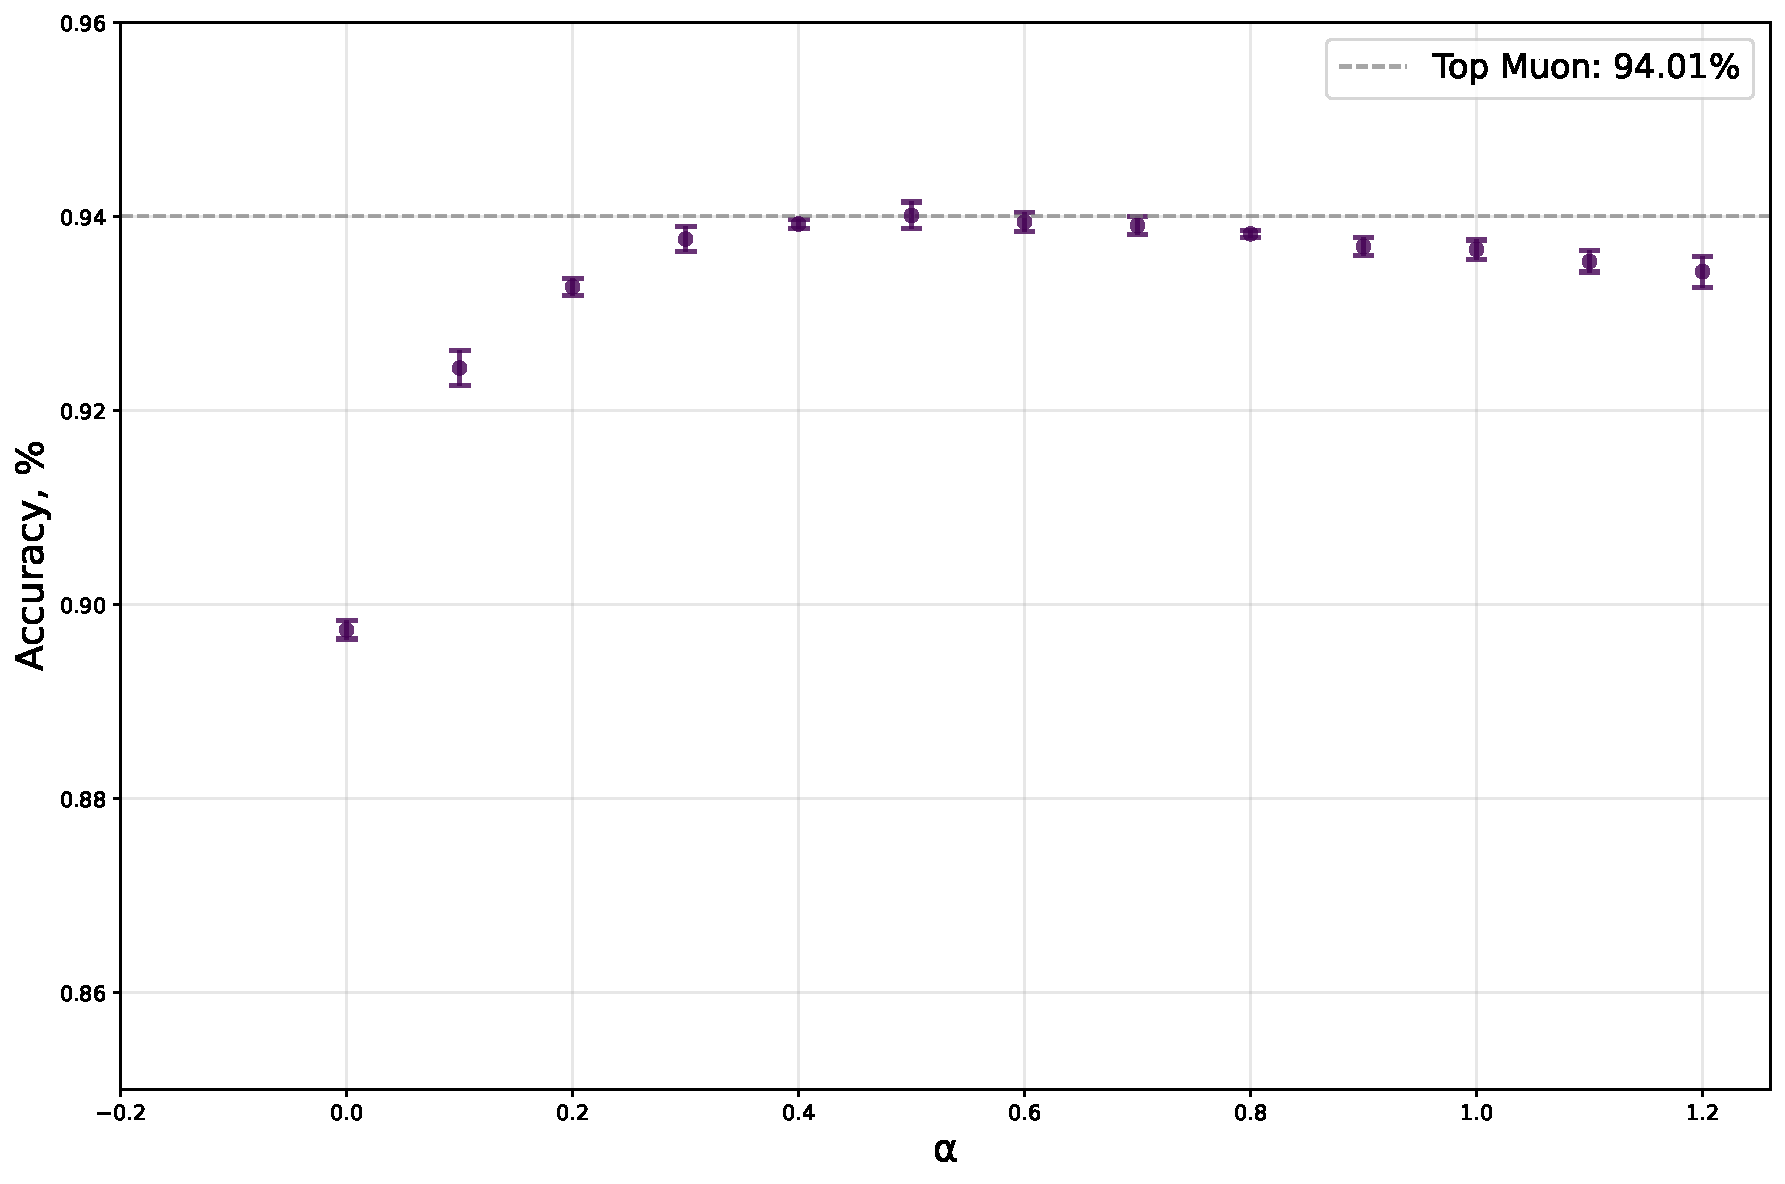
\includegraphics[width=\linewidth]{fmuon_tuned_diff_alpha.pdf}
        \centering
        \scriptsize With params tuned for F-Muon
      \end{column}
    \end{columns}
    \vspace{0.6em}
    \centering

    \footnotesize F-Muon with \(\alpha = 0.5\) matches Muon after tuning

    \faQuestionCircle \space How should we interpret cases with $\alpha > 1$?
  \end{frame}

%----------------------------------------
\begin{frame}{LMO balls on CIFAR-10}
  \begin{figure}[t]
    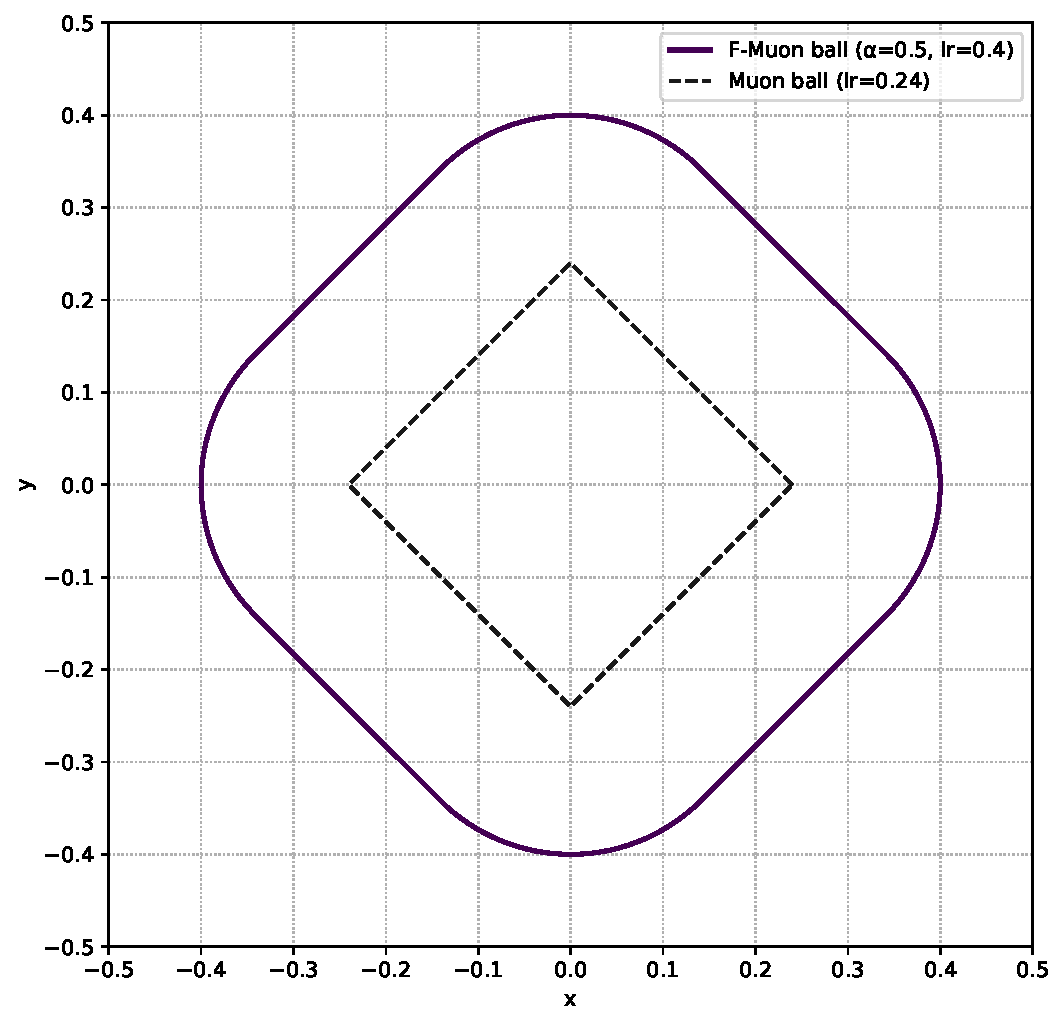
\includegraphics[height=0.7\textheight]{fstardual_cifar.pdf}
    \centering

    \footnotesize LMO balls for learning rates from the experiment

  \end{figure}
\end{frame}
%-----------------------------------------------------------------------------------------------
\begin{frame}{NanoGPT speedrun}
  Setup from \citet{modded_nanogpt_2024}: 1750 iterations and cross-entropy loss lower than 3.28
    \begin{itemize}
      \item Muon: {\tt lr=0.05, momentum=0.95}, final loss = 3.279
      \item F-Muon with \(\alpha=0.5\): {\tt lr=0.07, momentum=0.95}, final loss = 3.281
      \item NSGD: {\tt lr=0.07, momentum=0.96}, final loss = 3.4651
      \item F-Muon with $\alpha=0.5$: {\tt lr=0.07, momentum=0.96}, final loss = 3.2824!
    \end{itemize}
\end{frame}
%----------------------------------------------------------------------------------------------
\begin{frame}{Formal assumptions}
  L-smoothness:
  \begin{aequation}\label{eq:L}
    \norm{\nabla f(\mX) - \nabla f(\mX')}^\dagger \leq L \norm{\mX-\mX'}
    \quad\text{for all}\;
    \mX, \mX' \in \Rmn,
    \end{aequation}
  
  Bounded variance:
    \begin{aequation}\label{eq:variance}
      \Ed{\xi \sim \cD}{g(\mX;\xi)} = \nabla f(\mX)
      \quad\text{and}\quad
      \Ed{\xi \sim \cD}{\sqnf{g(\mX;\xi) - \nabla f(\mX)}} \leq \sigma^2
      \quad\text{for all}\;
      \mX \in \Rmn,
      \end{aequation}
  
  Bounded norm:
      \begin{aequation}\label{eq:norm}
        \norm{\mX}^\dagger \leq \rho\cdot\normf{\mX}
        \quad\text{for all}\;
        \mX \in \Rmn,
        \end{aequation}

  From Marchenko-Pastur law, $\normf{\cdot} \sim \frac{\sqrt{n}}{2}\norms{\cdot}$ and $\normn{\cdot} \sim \frac{n}{2}\norms{\cdot}$ for large $n$.
          
    

\end{frame}
\begin{frame}{Bounds from \citep{kovalev2025understanding}}
  \begin{lemma}\label{lemma:stoch_tr}
    To reach the precision $\E{\min_{k=1\ldots K} \norm{\nabla f(\mX_k)}^\dagger} \leq \epsilon$ under the assumptions \Cref{eq:L}, \Cref{eq:variance}, \Cref{eq:norm}, it is sufficient to choose the parameters as follows:
    \begin{align}
        \eta &= \cO\left(\min\left\{\frac{\epsilon}{L}, \frac{\epsilon^3}{\rho^2\sigma^2L}\right\}\right),
        \qquad
        \alpha = \cO\left(\min\left\{1, \frac{\epsilon^2}{\rho^2\sigma^2}\right\}\right),
        \\
        \label{eq:str_K_nonconvex}
        K &= \cO\left(\max\left\{
            \frac{\rho\sigma}{\epsilon},
            \frac{\rho^3\sigma^3}{\epsilon^3},
            \frac{L\Delta_0}{\epsilon^2},
            \frac{L\Delta_0\rho^2\sigma^2}{\epsilon^4}
        \right\}\right).
    \end{align}
    \end{lemma}

\end{frame}
%----------------------------------------
\begin{frame}{Random linear least squares: Loss and the Spectral Norm of the gradient}
  \begin{columns}[T,totalwidth=\textwidth]
    \begin{column}{0.48\textwidth}
      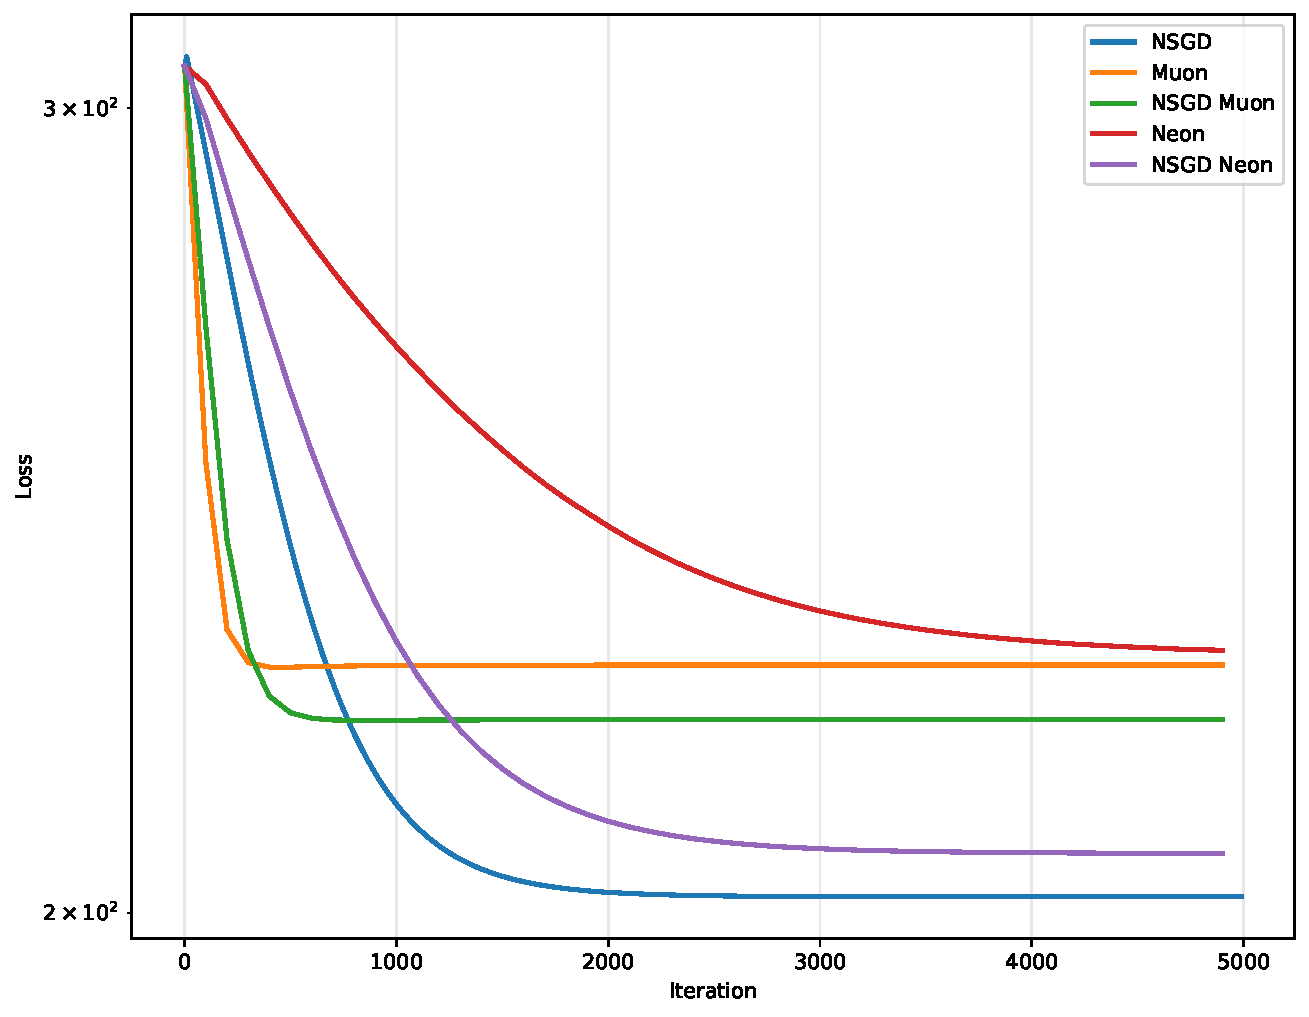
\includegraphics[width=\linewidth]{simple_lls/loss_vs_iteration_50x50.pdf}
      \centering
      \scriptsize Loss vs iteration
    \end{column}
    \begin{column}{0.48\textwidth}
      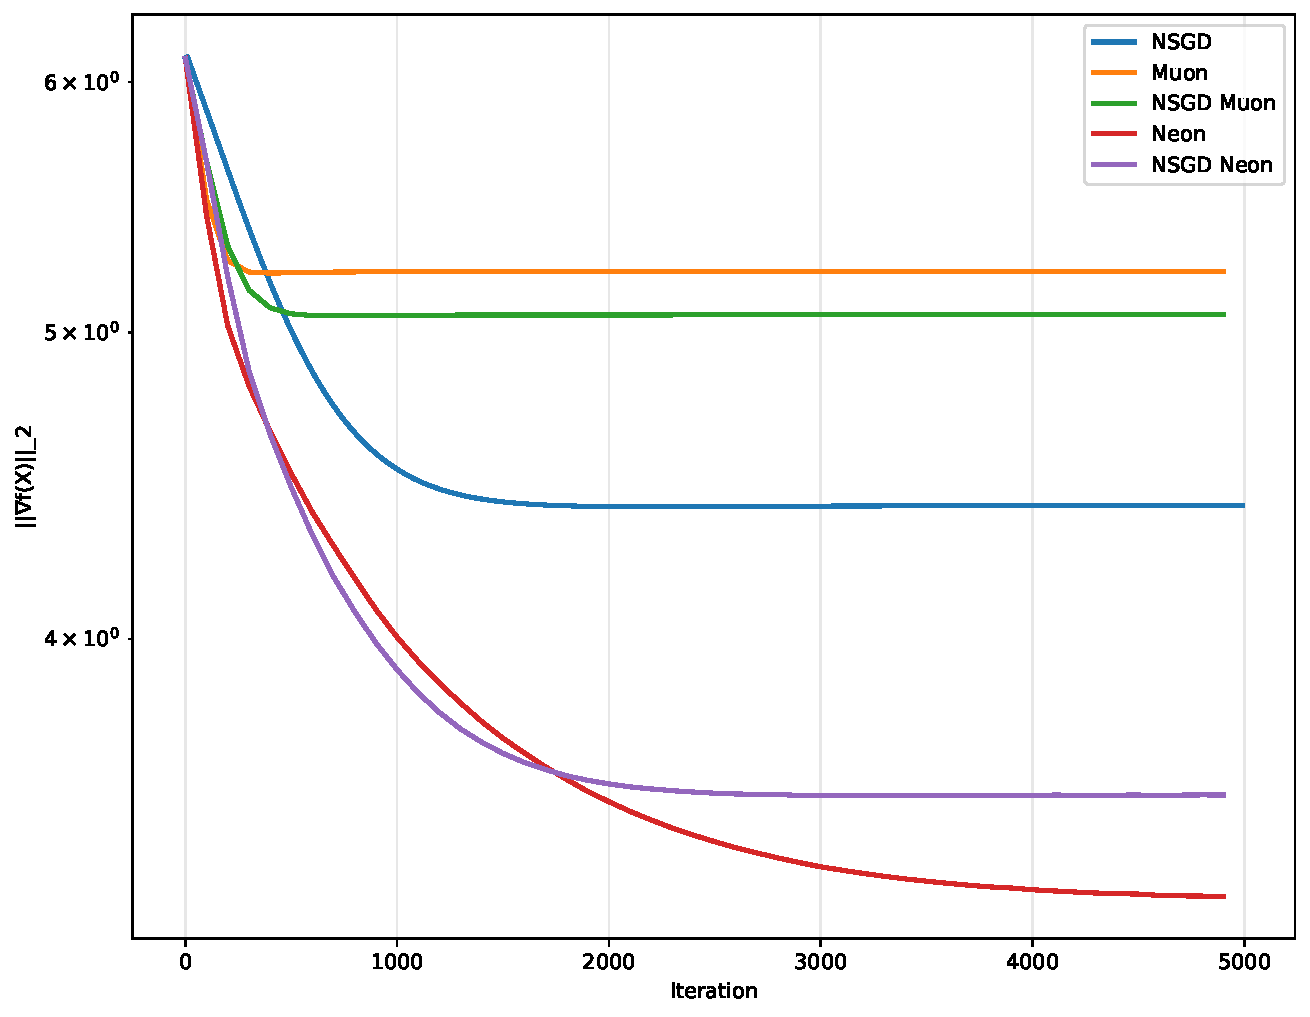
\includegraphics[width=\linewidth]{simple_lls/gradient_spectral_norm_vs_iteration_50x50.pdf}
      \centering
      \scriptsize Spectral norm of gradient vs iteration
    \end{column}
  \end{columns}
  \vspace{0.3em}
  \centering
  \footnotesize Linear least squares problem for a 50 x 50 matrix. Common {\tt lr=0.01}.
\end{frame}

%----------------------------------------
\begin{frame}{Geometric intuition: Ky Fan norms}
  \centering
  \begin{minipage}{0.46\textwidth}
      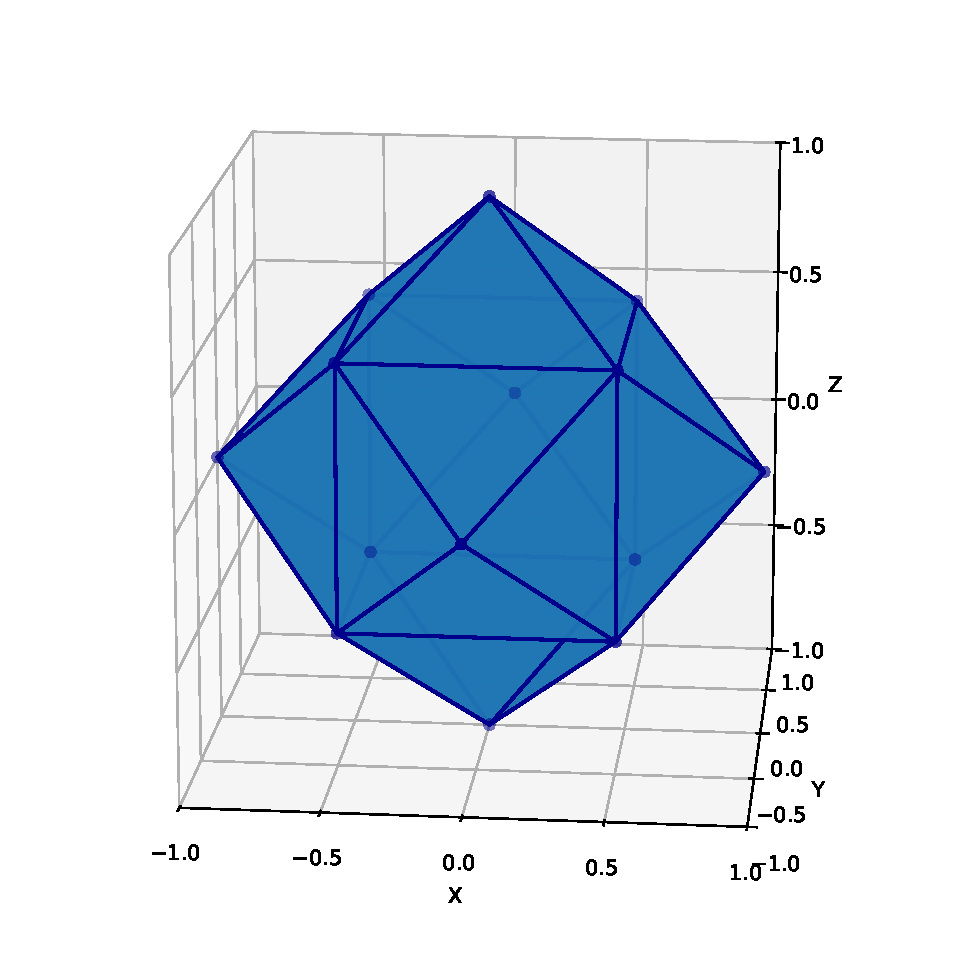
\includegraphics[height=0.75\textheight,keepaspectratio]{KyFan.pdf}
  \end{minipage}\hfill
  \begin{minipage}{0.46\textwidth}
      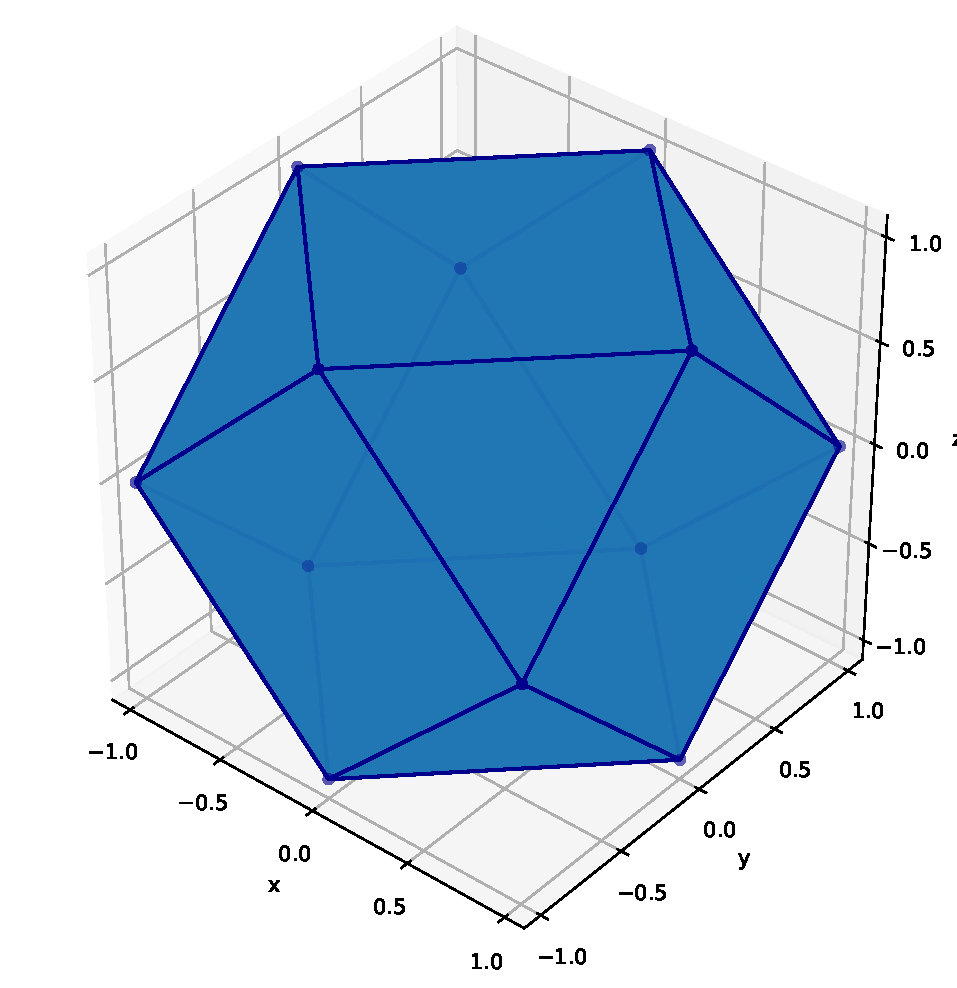
\includegraphics[height=0.75\textheight,keepaspectratio]{KyFanDual.pdf}
  \end{minipage}
  
  \vspace{0.3em}
  \footnotesize Ky Fan rank-2 ball and its dual in a 3D singular-value space
  \end{frame}
%----------------------------------------
\begin{frame}{Conclusions}
  \begin{itemize}
    \item Muon and NSGD are special cases of F-Fanions
    \item Mixture of norm-based updates is a norm-based update!
    \item No existing bounds describe the superiority of the spectral norm
  \end{itemize}

  \vspace{2em}
  \textbf{For future experiments}: Exploration of matrix and vector algorithms correspondence
\end{frame}

%----------------------------------------
\begin{frame}[allowframebreaks]{References}
  % Match article's bibliography style and entries
  \printbibliography
  %\bibliographystyle{../conf_article/icomp2024_conference}
  %\bibliography{../conf_article/icomp2024_conference}
\end{frame}

\end{document}


